\chapter{Development And Implementation}%
\label{chapter:development-and-implementation}

\begin{introduction}
Building upon the proposed framework, this chapter describes the practical development and implementation process undertaken. In this thesis, the specific tools, technologies, and configurations used to realize the solution are described, including the construction of key modules and the configuration of the experimental environment required for subsequent validation.
\end{introduction}

\section{Development Environment and Tools}

To construct and validate the proposed framework, a virtualized multi-\ac{VM} environment was orchestrated using Vagrant with VirtualBox as the provider. This approach allowed for the creation of a reproducible and isolated network testbed. The environment consists of four distinct \acp{VM}, each running Ubuntu 22.04 LTS (Jammy Jellyfish) as the base operating system. The roles and typical resource allocations for these \acp{VM}, as defined in the \texttt{Vagrantfile}, are:

\begin{enumerate}
    \item \textbf{\texttt{core} \ac{VM}:} Hosts the \ac{5GC} functions and the \ac{EAP} Authentication Server. Allocated 2\ac{GB} \ac{RAM} and 1 \ac{CPU}.

    \item \textbf{\texttt{gnb} \ac{VM}:} Runs the \ac{gNB} simulator. Allocated 1\ac{GB} \ac{RAM} and 1 \ac{CPU}.

    \item \textbf{\texttt{ue} \ac{VM}:} Represents the \ac{5G-RG}, acting as a \ac{UE} towards the \ac{5GC} and as an \ac{EAP} Authenticator/Gateway towards the \ac{NAUN3} device. Allocated 1\ac{GB} \ac{RAM} and 1 \ac{CPU}.

    \item \textbf{\texttt{naun3} \ac{VM}:} Simulates the Wi-Fi-only/\ac{NAUN3} end device, acting as an \ac{EAP} Supplicant. Allocated 1\ac{GB} \ac{RAM} and 1 \ac{CPU}.
\end{enumerate}

The following core software components and tools were utilized across these \acp{VM}, installed and configured via shell scripts executed during Vagrant provisioning:

\begin{enumerate}
    \item  {
        \textbf{\ac{5G} Network Simulation:}
        \begin{itemize}
            \item \textbf{Open5GS:} The open-source implementation of \ac{5GC} functions (\ac{AMF}, \ac{SMF}, \ac{UPF}, \ac{NRF}, \ac{AUSF}, \ac{UDM}, \ac{UDR}, \ac{PCF}, \ac{NSSF}). Installed on the \texttt{core} \ac{VM}.

            \item \textbf{MongoDB:} Used as the database backend for Open5GS, storing subscriber information and network function configurations. Installed from the official MongoDB repositories on the \texttt{core} \ac{VM}.

            \item \textbf{UERANSIM:} An open-source \ac{gNB} and \ac{UE} simulator. Cloned from its GitHub repository and compiled from source on the \texttt{gnb} \ac{VM} (for \ac{gNB} functionality) and the \texttt{ue} \ac{VM} (for \ac{UE}/\ac{5G-RG} functionality). The \texttt{nr-cli} utility from UERANSIM was also made available
        \end{itemize}
    }

    \item {
        \textbf{Authentication Infrastructure:}
        \begin{itemize}
            \item \textbf{FreeRADIUS:} Employed as the \ac{EAP-TLS} Authentication Server. Installed on the \texttt{core} \ac{VM} and configured to handle \ac{EAP-TLS}, manage client (\ac{UE}/\ac{5G-RG}) definitions, and generate/use X.509 certificates.

            \item \textbf{\texttt{hostapd}:} Utilized as the \ac{EAP} Authenticator on the \texttt{ue} \ac{VM} (\ac{5G-RG}). Cloned from its official repository (\texttt{w1.fi/hostap.git}) and compiled from source with the \texttt{CONFIG\_DRIVER\_WIRED=y} option enabled to support \ac{EAP} over wired interfaces for the \ac{NAUN3} device connection.

            \item \textbf{\texttt{wpa\_supplicant}:} Used as the \ac{EAP} Supplicant on the \texttt{naun3} \ac{VM}. Installed via \texttt{apt} and configured to perform \ac{EAP-TLS} authentication using client certificates.
        \end{itemize}
    }

    \item {
        \textbf{Networking and Utility Tools:}
        \begin{itemize}
            \item \textbf{\texttt{dnsmasq}:} Configured as a \ac{DHCP} server on the \texttt{ue} \ac{VM} to provide \ac{IP} addresses to \ac{NAUN3} devices connecting to its local network interface (\texttt{enp0s9}).

            \item \textbf{\texttt{yq}:} A command-line YAML processor, installed via \texttt{snap}. Extensively used in provisioning scripts to modify Open5GS and UERANSIM configuration files (e.g., setting \ac{IP} addresses, \acp{DNN}, \acp{APN}).

            \item \textbf{Build Tools:} \texttt{make}, \texttt{git}, \texttt{gcc}, \texttt{g++}, \texttt{cmake} (via \texttt{snap}), \texttt{libsctp-dev}, \texttt{lksctp-tools}, \texttt{pkgconf}, \texttt{libssl-dev}, \texttt{libnl-3-dev}, \texttt{libnl-genl-3-dev} were installed for compiling UERANSIM and \texttt{hostapd} from source.

            \item \textbf{System Utilities:} \texttt{iproute2}, \texttt{net-tools}, \texttt{curl}, \texttt{gnupg} were used for network configuration and repository management.

            \item \textbf{Node.js and Nginx:} Installed on the \texttt{core} \ac{VM} to support and expose the Open5GS WebUI.
        \end{itemize}
    }

    \item {
        \textbf{Custom Tools and Scripts}
        \begin{itemize}
            \item \textbf{\texttt{open5gs-dbctl}:} A shell script provided and used on the \texttt{core} VM to interact with the MongoDB database for managing Open5GS subscriber entries (adding \acp{UE}, defining \acp{APN} and slices).

            \item \textbf{\texttt{interceptor}:} A custom Go application (compiled from source located in an \texttt{interceptor} directory, as indicated in the \texttt{Vagrantfile}) deployed on the \texttt{ue} \ac{VM}. This is the key tool developed to orchestrate the logic for monitoring \texttt{hostapd} events and managing \ac{PDU} sessions. It's specific internal workings are detailed later.

            \item \textbf{Provisioning Scripts:} A set of shell scripts (\texttt{core\_install}, \texttt{gnb\_install}, \texttt{ue\_install}, \texttt{naun3\_install}, \texttt{auth\_server\_install}, \texttt{ueransim\_install}) were used by Vagrant to automate the installation and configuration of all software components on their respective \acp{VM}.
        \end{itemize}
    }
\end{enumerate}

\subsection{Network Topology and Configuration Management}

\begin{figure}
    \centering
    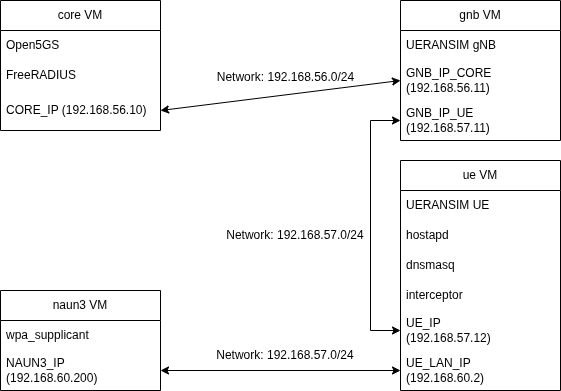
\includegraphics[width=0.75\linewidth]{figs/topology_vagrant_machine_topology.png}
    \caption{Vagrant deployed \acp{VM} with respecting services and interconnecting networks topology}
    \label{fig:topology_vagrant_machine_topology}
\end{figure}

The \texttt{Vagrantfile} defines several private networks (see Figure \ref{fig:topology_vagrant_machine_topology}) to interconnect the \acp{VM}, establishing distinct network segments for communication between the \ac{5GC} and \ac{gNB} (\texttt{192.168.56.0/24}), \texttt{gNB} and \ac{UE}/\ac{5G-RG} (\texttt{192.168.57.0/24}), and the \ac{UE}/\ac{5G-RG}'s local network for \ac{NAUN3} devices (\texttt{192.168.60.0/24}). \ac{IP} addresses for various interfaces and services (e.g., \texttt{CORE\_IP}, \texttt{GNB\_IP\_CORE}, \texttt{UE\_LAN\_IP}, \texttt{AUTH\_SERVER\_IP} for \ac{RADIUS} communication over the \texttt{backhaul} tunnel) are explicitly defined and passed as arguments to the provisioning scripts.

Vagrant's synced folder feature was utilized to share:

\begin{itemize}
    \item \ac{EAP}/\ac{RADIUS} certificates generated by FreeRADIUS on the \texttt{core} \ac{VM} to the \texttt{naun3} \ac{VM} (via \texttt{/certs} on the guest).

    \item Runtime logs from all \acp{VM} to a \texttt{./build/runtime-logs} directory on the host machine.

    \item The compiled \texttt{interceptor} binary to the \texttt{ue} \ac{VM}.
\end{itemize}

This comprehensive setup provides a fully functional, albeit simulated, environment for developing and testing the proposed solution for integrating \ac{NAUN3} devices into a \ac{5G} network.

\section{Implementation of Proposed Authentication Logic}

This section details the practical implementation of the \ac{EAP-TLS} authentication mechanism, which forms the first crucial step in integrating \ac{NAUN3} devices. The setup involves configuring an \ac{EAP} Authentication Server (FreeRADIUS), an Authenticator (\texttt{hostapd} on the \ac{5G-RG}), and an \ac{EAP} Supplicant (\texttt{wpa\_supplicant} on the \ac{NAUN3} device), with a custom Go application (\texttt{interceptor}) orchestrating the events on the \ac{5G-RG}.

Firstly, the \ac{EAP} Authentication Server was implemented using FreeRADIUS on the \texttt{core} \ac{VM}, provisioned by the \texttt{auth\_server\_install} script. This script is responsible for configuring FreeRADIUS and they keys it uses.

Regarding \ac{RADIUS} Client Configuration, the \ac{5G-RG} (\texttt{ue} \ac{VM}) was registered as a \ac{RADIUS} client in \texttt{/etc/freeradius/3.0/clients.conf}. This entry specified the \texttt{ue} \ac{VM}'s \ac{IP} address designated for \ac{EAP} traffic (the \texttt{CLIENT\_EAP\_IP} variable defined in the \texttt{Vagrantfile} as \texttt{10.45.0.2}) and a shared secret (the \texttt{CLIENT\_SECRET} variable also defined in the \texttt{Vagrantfile}, holding a randomly generated value) for securing \ac{RADIUS} communication.

FreeRADIUS provides the mechanisms necessary to generate a \ac{PKI} via a script which generates the following:

\begin{itemize}
    \item A \ac{CA} certificate (\texttt{ca.pem})
    \item A server certificate (\texttt{server.pem}) and private key (\texttt{server.key}) for FreeRADIUS itself.
    \item A client certificate (\texttt{client.p12}, a \ac{PKCS12} bundle containing the certificate and private key) for the \ac{NAUN3} device. Passwords for these certificates (\texttt{CERT\_CA\_PASSWD}, \texttt{CERT\_SERVER\_PASSWD}, \texttt{CERT\_CLIENT\_PASSWD}) are randomly generated value in the \texttt{Vagrantfile} and passed to the script.
\end{itemize}

Also, the \ac{EAP} module in FreeRADIUS (\texttt{/etc/freeradius/3.0/mods-available/eap}) was to modified such as:

\begin{itemize}
    \item To set the \ac{EAP} type to \ac{TLS} - \texttt{default\_eap\_type = tls}.
    \item The server's private key password is set - \texttt{private\_key\_password}
    \item The paths for the certificates and private keys are set - \texttt{private\_key\_file}, \texttt{certificate\_file} and \texttt{ca\_file}
\end{itemize}

The necessary certificates for the \ac{NAUN3} device (\ac{CA} certificate \texttt{ca.pem} and the client \ac{PKCS12} bundle \texttt{client.p12}) were copied from the \texttt{core} \ac{VM}'s FreeRADIUS certificate directory to a Vagrant synced folder, making them accessible to the \texttt{naun3} \ac{VM}.

Secondly, the \ac{5G-RG} (\texttt{ue} \ac{VM}) acts as the \ac{EAP} Authenticator, using \texttt{hostapd}. Its setup is managed by the \texttt{ue\_install} script.

Starting installation, \texttt{hostapd} is cloned from \texttt{w1.fi/hostap.git} and compiled from source, ensuring the \texttt{CONFIG\_DRIVER\_WIRED=y} option was enabled in its \texttt{.config} file to support \ac{EAP} authentication over the virtual interface connecting both the \texttt{ue} \ac{VM} to the \texttt{naun3} \ac{VM}.

Regarding the \texttt{hostadp} configuration, which is the entity responsible for \ac{LAN} authentication, we can review it bellow (see Code Snippet \ref{lst:hostapd-configurations}).

\begin{lstlisting}[caption=hostapd configurations,label={lst:hostapd-configurations}]
interface=enp0s9
driver=wired
ctrl_interface=/var/run/hostapd
ctrl_interface_group=vagrant

logger_syslog=-1
logger_syslog_level=0

ieee8021x=1 
own_ip_addr=$CLIENT_EAP_IP

auth_server_addr=$AUTH_SERVER_IP
auth_server_port=1812
auth_server_shared_secret=$CLIENT_SECRET
\end{lstlisting}

\begin{itemize}
    \item \texttt{auth\_server\_addr}: Set to \texttt{AUTH\_SERVER\_IP} (the \ac{IP} of the \texttt{core} \ac{VM} (10.45.0.1) reachable via the \texttt{backhaul} \ac{PDU} session).
    \item \texttt{auth\_server\_port=1812}.
    \item \texttt{auth\_server\_shared\_secret}: Set to \texttt{CLIENT\_SECRET}.
    \item \texttt{own\_ip\_addr}: Set to \texttt{CLIENT\_EAP\_IP} (10.45.0.2), ensuring \ac{RADIUS} packets from \texttt{hostapd} originate from the correct \ac{IP} address within the \texttt{backhaul} \ac{PDU} session
\end{itemize}

When implementing the \texttt{naun3} device, it configured to act as an \ac{EAP} Supplicant using \texttt{wpa\_supplicant}, as detailed in the \texttt{naun3\_install} installation script.

Going through the configurations in Code Snippet \ref{lst:wpa-supplicant-configurations} we can see the following.

\begin{lstlisting}[caption=wpa\_supplicant configurations,label={lst:wpa-supplicant-configurations}]
ctrl_interface=DIR=/var/run/wpa_supplicant GROUP=vagrant
eapol_version=2
ap_scan=0

network={
    eapol_flags=0

    key_mgmt=IEEE8021X
    eap=TLS

    identity="user@example.org"
    ca_cert="/certs/ca.pem"
    private_key="/certs/client.p12"
    private_key_passwd="$CERT_CLIENT_PASSWD"
}
\end{lstlisting}

A network block was defined specifically for \ac{EAP-TLS} authentication:

\begin{itemize}
    \item \texttt{key\_mgmt=IEEE8021X}.
    \item \texttt{eap=TLS}.
    \item \texttt{identity="user@example.org"} was used as the \ac{EAP} identity.
    \item \texttt{ca\_cert="/certs/ca.pem"} specified the path to the \ac{CA} certificate (obtained via the synced folder).
    \item \texttt{private\_key="/certs/client.p12"} specified the path to the client's \ac{PKCS12} certificate/key bundle.
    \item \texttt{private\_key\_passwd} was set to \texttt{CERT\_CLIENT\_PASSWD}.
\end{itemize}

Also, \texttt{wpa\_supplicant} was configured to use the wired driver (via the \texttt{-Dwired} argument) for its network interface (via the \texttt{-ienp0s8} argument).The scan for \acp{AP} is also disabled via \texttt{ap\_scan=0}, which is appropriate for wired connections.

When it comes to orchestrating the authentication events, the custom Go application, \texttt{interceptor.go}, deployed on the \texttt{ue} \ac{VM}, plays a pivotal role in bridging the \ac{EAP} authentication outcome with the \ac{5G} session management logic.

In it s interaction with \texttt{hostapd}, the \texttt{interceptor} establishes a connection to \texttt{hostapd}'s control interface socket (e.g., \texttt{/var/run/hostapd/enp0s9}) using a Unix domain socket. It sends an \texttt{"ATTACH"} command to subscribe to \texttt{hostapd} events, and the \texttt{HostapdListener} goroutine continuously monitors messages from \texttt{hostapd}.

To detect \ac{EAP} successes, it specifically parses incoming messages for the string \texttt{"CTRL-EVENT-EAP-SUCCESS"}. An when one is detected,  the \texttt{interceptor} extracts the \ac{MAC} address of the authenticated \ac{NAUN3} device from the event message (e.g., \texttt{CTRL-EVENT-EAP-SUCCESS aa:bb:cc:dd:ee:ff}). This serves as a primary trigger for the \texttt{interceptor} that then proceeds to manage the device in its \texttt{allowed\_devices} map and initiates the logic for establishing a new \ac{PDU} session for this device.

\subsection{Implemented \ac{EAP-TLS} Authentication Flow Summary}

The implemented authentication sequence is as follows:

\begin{enumerate}
    \item The \texttt{naun3} \ac{VM} (\texttt{wpa\_supplicant}) attempts to authenticate over its \texttt{enp0s8} interface connected to the \texttt{ue} \ac{VM}'s (\ac{5G-RG}) \texttt{enp0s9} interface.
    \item \texttt{hostapd} on the \texttt{ue} \ac{VM} detects the \ac{EAPOL}-Start and initiates the \ac{EAP-TLS} exchange.
    \item \ac{EAP-TLS} messages are relayed by \texttt{hostapd} to the FreeRADIUS server on the \texttt{core} \ac{VM}. This communication occurs via \ac{RADIUS} packets, which are transported over the \ac{5G-RG}'s \texttt{backhaul} \ac{PDU} session (using \texttt{CLIENT\_EAP\_IP} as the source and \texttt{AUTH\_SERVER\_IP} as the destination).
    \item FreeRADIUS validates the \ac{NAUN3} device's client certificate against its \ac{CA} and configuration.
    \item Upon successful validation, FreeRADIUS sends a \ac{RADIUS} Access-Accept containing an \ac{EAP}-Success message back to \texttt{hostapd}.
    \item \texttt{hostapd} relays the \ac{EAP}-Success to \texttt{wpa\_supplicant} on the \ac{NAUN3} device and concurrently emits the \texttt{CTRL-EVENT-EAP-SUCCESS <NAUN3\_MAC\_ADDRESS>} message to its control interface.
    \item The \texttt{interceptor} application on the \texttt{ue} \ac{VM} captures this event, confirming the \ac{NAUN3} device's successful local authentication and readiness for the next stage of network integration.
\end{enumerate}

This setup effectively implements the \ac{EAP-TLS} authentication flow, using standard tools configured to interact in a specific way, with the custom interceptor acting as the crucial link to the \ac{5G}-specific actions.

\section{Implementation of Identity Management Mechanisms}

With local \ac{EAP-TLS} authentication successfully implemented, this section details how the framework manages a unique network presence for each authenticated \ac{NAUN3} device. Given that these devices lack native \ac{5G} identifiers (\ac{SUPI}/\ac{SUCI}), the core of the implemented solution is the dynamic establishment and management of a dedicated \ac{PDU} Session by the \ac{5G-RG} for each \ac{NAUN3} device. This \ac{PDU} Session effectively serves as its proxy identity within the \ac{5G} network. The custom Go application, running on the \ac{5G-RG} (\texttt{ue} \ac{VM}), is the central orchestrator of this mechanism.

\subsection{1. Triggering Proxy Identity Establishment}

The process of establishing a proxy identity for an \ac{NAUN3} device is initiated immediately after its successful local authentication. The \texttt{HostapdListener} \textit{goroutine} (defined in \texttt{hostapd\_interceptor.go} and launched by \texttt{main.go} monitors \texttt{hostapd}'s control interface. Upon detecting the \texttt{CTRL-EVENT-EAP-SUCCESS <MAC\_ADDRESS>} message (constant \texttt{hostapdEventEAPSuccess}), the listener extracts the \ac{MAC} address of the successfully authenticated \ac{NAUN3} device. This event and the device's \ac{MAC} address serve as the trigger for the subsequent identity management steps.

\subsection{2. \acs{PDU} Session Creation by the Orchestration Logic}

Once an \ac{NAUN3} device is authenticated, the \texttt{HostapdListener} calls the \texttt{NewPDUSession} function (from \texttt{ueransim\_pdu\_handler.go}. This function is responsible for requesting a new \ac{PDU} session from the \ac{5GC} via the \ac{5G-RG}'s \ac{UE} stack (UERANSIM).

\begin{itemize}
    \item{ 
        It constructs and executes the UERANSIM command-line interface tool: \texttt{nr-cli <5G-RG\_IMSI> --exec "ps-establish IPv4 --sst 1 --dnn <DNN\_NAME>"}.
        \begin{itemize}
            \item The \texttt{<5G-RG\_IMSI>} (e.g., 999700000000001) is the pre-configured \ac{IMSI} of the \ac{5G-RG} itself, passed as a command-line argument (\texttt{--imsi}) to the main application and subsequently to the \texttt{HostapdListener} and \texttt{NewPDUSession}.
            \item The \texttt{<DNN\_NAME>} (e.g., \texttt{clients}) is also passed as a command-line argument (\texttt{--dnn}) and used to target the \ac{PDU} session request. This \ac{DNN} was specifically configured in Open5GS on the \texttt{core} \ac{VM} and made known to the UERANSIM \ac{UE} stack on the \texttt{ue} \ac{VM}.
        \end{itemize}
    }
    \item After requesting the session, \texttt{NewPDUSession} enters a polling loop, repeatedly calling \texttt{LastPDUSession} (which executes \texttt{nr-cli <5G-RG\_IMSI> --exec "ps-list"} and parses its YAML output) until the newly requested session transitions to the \texttt{"PS-ACTIVE"} state (\texttt{pduSessionStateActive}) and has an \ac{IP} address assigned by the \ac{5GC}. A timeout mechanism with retries (\texttt{pduSessionEstablishRetries}, \texttt{pduSessionEstablishInterval}) is implemented.
\end{itemize}

\subsection{3. Gateway-Managed Internal Mapping}

The main application maintains a global map: \texttt{allowedDevices} which is a key-value map, that identifies \texttt{Device} objects using their \ac{MAC} addresses as keys. This \texttt{Device} object (defined in \texttt{network\_handler.go}) stores the state.

\begin{itemize}
    \item When an \ac{NAUN3} device successfully authenticates and its dedicated \ac{PDU} session (type \texttt{Session} from \texttt{ueransim\_pdu\_handler.go}) becomes active, an entry is added to this map by the \texttt{HostapdListener}. The \ac{MAC} address of the \ac{NAUN3} device serves as the key.
    
    \item The \texttt{Device} object stores crucial information: its current \texttt{state} (e.g., "AUTHENTICATED", "LEASED", "REACHABLE"), a pointer to the \texttt{Session} object (containing \ac{PDU} Session ID, state, \ac{APN}/\ac{DNN}, and the \ac{5GC}-allocated \ac{IP} Address), Lease information (from \texttt{dnsmasq\_handler.go}, and \texttt{AppliedIPTablesRules} (a slice of \texttt{AppliedRuleDetail} from \texttt{routing\_handler.go}. This map is central to linking the local device to its \ac{5G} network representation and its specific traffic routing rules.
\end{itemize}

\subsection{4. \ac{NAUN3} Device Local \ac{IP} Addressing}

For the \ac{NAUN3} device to communicate on the local network segment:

\begin{itemize}
    \item Upon successful \ac{PDU} session establishment, the \texttt{HostapdListener} calls \texttt{AllowMAC()} (from \texttt{dnsmasq\_handler.go}). This function appends \texttt{dhcp-host=<NAUN3\_MAC\_ADDRESS>,<LEASE\_TIME>,set:known} to \texttt{/etc/allowed-macs.conf} on the \ac{5G-RG} (\texttt{ue} \ac{VM}). The \texttt{leaseTime} is passed as a command-line argument (\texttt{--lease-time}) to \texttt{main.go}.

    \item \texttt{dnsmasq} on the \ac{5G-RG} (configured in \texttt{ue\_install}) serves \ac{DHCP} only to \ac{MAC} addresses listed as \texttt{"known"} in this file.

    \item \texttt{wpa\_supplicant} on the \ac{NAUN3} \ac{VM} then executes \texttt{sudo dhclient enp0s8} to obtain a local \ac{IP} address (e.g., from 192.168.60.0/24).
\end{itemize}

\subsection{5. Proxy Identity Lifecycle Management (Termination)}

The \texttt{HostDisconnectListener} \textit{goroutine} (in \texttt{network\_handler.go}, launched by \texttt{main.go}) and the \texttt{ForgetDevice} function (in \texttt{network\_handler.go}) manage the termination of the proxy identity.

\begin{itemize}
    \item \texttt{HostDisconnectListener} periodically checks device reachability on the \ac{LAN} interface (e.g., \texttt{enp0s9}, derived from the \texttt{--interface} flag passed to \texttt{main.go}) using \texttt{netlink.NeighList} (which is based on the \texttt{ip neighbour} too). A device is considered for removal if its state becomes stale/failed and its \ac{DHCP} lease is significantly into its expiry, or if the \ac{MAC} is no longer in the \ac{ARP}/neighbor list.

    \item{
        This triggers the \texttt{ForgetDevice} function, which performs cleanup:
        \begin{itemize}
            \item \texttt{DisallowMAC()} (from dnsmasq\_handler.go): Removes the \ac{NAUN3} device's \ac{MAC} address entry from the \texttt{allowedMACsFilePath} and the \texttt{leasesFilePath} (passed via \texttt{--leases} flag to \texttt{main.go}), followed by a \texttt{RestartDnsmasq()} call which will force \texttt{dnsmasq} to restart and thus reload the configurations now updated.

            \item \texttt{Deauth()} (from \texttt{hostapd\_interceptor.go}): Sends a \texttt{"DEAUTHENTICATE <MAC\_ADDRESS>"} command to \texttt{hostapd}.

            \item \texttt{ruleManager.RemoveRulesForDevice()} (from \texttt{routing\_handler.go}): Removes the specific \texttt{iptables} rules and \texttt{ip route/rule} entries that were previously applied for this device, using the \texttt{AppliedIPTablesRules} stored in the \texttt{Device} object. The \texttt{ruleManager} is initialized in \texttt{main.go}.

            \item \texttt{ReleasePDUSession()} (from \texttt{ueransim\_pdu\_handler.go}): Executes \texttt{nr-cli <5G-RG\_IMSI> --exec "ps-release <PDU\_SESSION\_ID>"} to terminate the dedicated clients \ac{PDU} session associated with this \ac{NAUN3} device.

            \item Finally, the \ac{NAUN3} device's entry is removed from the global \texttt{allowedDevices} map.
        \end{itemize}
    }

    \item The \texttt{DnsmasqListener} (in \texttt{dnsmasq\_handler.go}, launched by \texttt{main.go}) also monitors the \ac{DHCP} lease file (\texttt{leasesFilePath}), updating lease details (\texttt{expiration}, \texttt{counter}) and transitioning the device state to \texttt{"LEASED"} within the \texttt{allowedDevices} map upon lease acquisition/renewal.
\end{itemize}

\subsection{6. Implemented Traffic Mapping}

The \texttt{interceptor} system, through the \texttt{routing\_handler.go} module, implements concrete traffic mapping for each authenticated \ac{NAUN3} device (as shown in Figure \ref{fig:policy-based-routing}), ensuring its traffic is routed via its dedicated \ac{PDU} session.

\begin{figure}
    \centering
    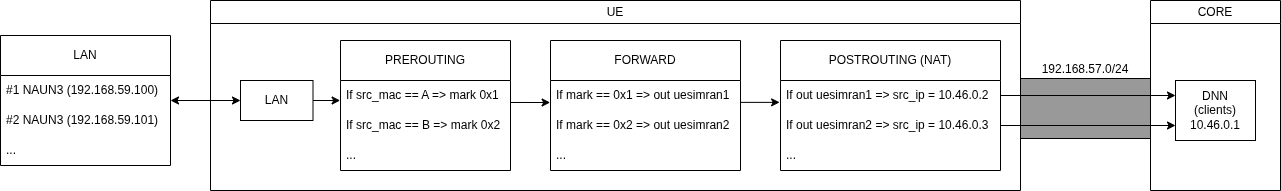
\includegraphics[width=1\linewidth]{figs/topology-Policy Based Routing.png}
    \caption{Policy Based Routing}
    \label{fig:policy-based-routing}
\end{figure}

\begin{itemize}
    \item After a \ac{PDU} session is successfully established for an \ac{NAUN3} device, the \texttt{HostapdListener} calls \texttt{ruleManager.ApplyMappingRules()}. The \texttt{ruleManager} instance is initialized in \texttt{main.go} via \texttt{NewRuleManager()}.

    \item \texttt{ApplyMappingRules} is passed the \ac{LAN} interface name (e.g., \texttt{enp0s9}, from \texttt{--lan-if} flag), the \ac{NAUN3}'s \ac{MAC} address, the \ac{PDU} session's tunnel interface name (e.g., \texttt{uesimtun<ID>}, where \texttt{ID} is the \ac{PDU} session ID), the \ac{PDU} session's gateway \ac{IP} (e.g., \texttt{10.46.0.1} for the \texttt{clients} \ac{DNN}, from \texttt{--pdu-gw-ip} flag ), and the \ac{PDU} session \texttt{ID}.
    
    \item{ 
        The function then systematically configures policy-based routing and \ac{NAT} using \texttt{iptables} and \texttt{ip} commands:
        
        \begin{enumerate}
            \item \textbf{Custom Routing Table:} An entry for a new routing table (e.g., \texttt{200+<PDU\_ID> table\_pdu\_<PDU\_ID>}) is added to \texttt{/etc/iproute2/rt\_tables} using the \texttt{manageRTTableEntry} function. This ensures the table definition persists.
            
            \item \textbf{Default Route in Custom Table:} A default route \texttt{ip route add default via <PDU\_GATEWAY\_IP> dev <PDU\_IF\_NAME> table table\_pdu\_<PDU\_ID>} is added, directing all traffic for this custom table out through the \ac{NAUN3}'s specific \ac{PDU} session interface.
            
            \item \textbf{Policy Rule:} An \ac{IP} policy rule \texttt{ip rule add fwmark <PDU\_ID> table table\_pdu\_<PDU\_ID>} is created. This rule directs any packet marked with the \ac{PDU} session ID (as a firewall mark) to use the newly created custom routing table.
            
            \item \textbf{Packet Marking:} An \texttt{iptables} rule is inserted into the \texttt{mangle} table's \texttt{PREROUTING} chain: \texttt{-i <LAN\_IF> -m mac --mac-source <NAUN3\_MAC> -j MARK --set-mark <PDU\_ID>}. This rule marks all incoming packets from the specific \ac{NAUN3} device's \ac{MAC} address on the \ac{LAN} interface with its corresponding \ac{PDU} session ID.
            
            \item \textbf{Forwarding:} An \texttt{iptables} rule in the \texttt{filter} table's \texttt{FORWARD} chain explicitly allows marked packets originating from the \ac{NAUN3}'s \ac{MAC} on the \ac{LAN} interface to be forwarded to its designated \ac{PDU} session interface: \texttt{-i <LAN\_IF> -o <PDU\_IF\_NAME> -m mac --mac-source <NAUN3\_MAC> -m mark --mark <PDU\_ID> -j ACCEPT}. A global \texttt{FORWARD} policy of \texttt{DROP} is assumed or set by \texttt{NewRuleManager}.
            
            \item \textbf{\ac{NAT} (Masquerade):} An \texttt{iptables} rule in the \texttt{nat} table's \texttt{POSTROUTING} chain: \texttt{-o <PDU\_IF\_NAME> -j MASQUERADE} performs \ac{SNAT} for all traffic exiting via the \ac{PDU} session interface, making it appear to originate from the \ac{IP} address assigned to that \ac{PDU} session.
        \end{enumerate}
    }
    
    \item These dynamically applied rules ensure that traffic from each authenticated \ac{NAUN3} device is uniquely marked, routed through its dedicated \ac{PDU} session, and correctly \textit{NATted} for external communication. The details of these applied rules are stored in the \texttt{Device.AppliedIPTablesRules} slice and are systematically removed by \texttt{ruleManager.RemoveRulesForDevice()} during the \texttt{ForgetDevice} process to ensure a clean state.
    
\end{itemize}

\section{Adaptation of Network Functions}

The successful implementation of the proposed framework did not require code-level modifications to the standard \ac{5G} \acp{NF} or \ac{RAN}/\ac{UE} simulators. Instead, these components were adapted through specific configurations to support the gateway-centric authentication and identity management scheme for \ac{NAUN3} devices. The primary tools used for this were \Open5GS for the \ac{5GC}, UERANSIM for the \ac{gNB} and the \ac{5G-RG}'s \ac{UE} stack, all provisioned and configured via scripts within a Vagrant-managed virtualized environment.

\subsection{Open5GS (\ac{5GC}) on \texttt{core} \ac{VM}}

The Open5GS components whose configurations were specifically adapted for this framework were the \ac{AMF}, \ac{SMF}, and \ac{UPF}. The \ac{AUSF} and \ac{UDM} operated in a standard manner for the \ac{5G-RG}'s own registration and authentication. The relevant configurations were applied as follows.

\begin{itemize}
    \item \textbf{Connectivity Configuration:} The \ac{AMF}'s \ac{NGAP} interface and the \ac{UPF}'s \ac{GTP-U} interface were bound to a designated \ac{IP} address on the \texttt{core} \ac{VM}, facilitating connectivity with the \ac{gNB} over their respective private network segment. This was achieved by modifying \texttt{amf.yaml} and \texttt{upf.yaml} configuration files using \texttt{yq}.

    \item{
        \textbf{\ac{DNN} Configuration:} Two distinct \acp{DNN} were defined in the \ac{SMF} and \ac{UPF} configurations to segregate traffic:

        \begin{itemize}
            \item \texttt{backhaul} \ac{DNN}: Configured in \texttt{smf.yaml} and \texttt{upf.yaml}, associated with the default \texttt{ogstun} tunnel interface. This \ac{DNN} provides the primary \ac{PDU} session for the \ac{5G-RG} itself, used for operational traffic such as \ac{RADIUS} communication with the \ac{EAP} Authentication Server. The \ac{SMF} configuration for this \ac{DNN} assigns \ac{IP}s from a dedicated subnet; the \ac{5G-RG}'s \ac{UE} stack is configured to use an \ac{IP} from this subnet for \ac{EAP} client communication, and the \ac{EAP} server on the \texttt{core} \ac{VM} is also reachable via an \ac{IP} in this same \texttt{backhaul} network space.

            \item \texttt{clients} \ac{DNN}: Also configured in \texttt{smf.yaml} and \texttt{upf.yaml}. A dedicated tunnel interface (\texttt{clientun0}) was created on the \texttt{core} \ac{VM} and assigned an \ac{IP} address to serve a distinct subnet. The \texttt{clients} \ac{DNN} was associated with this interface and subnet, enabling the \ac{SMF}/\ac{UPF} to allocate \acp{IP} from this specific range for the individual \ac{PDU} sessions established for each \ac{NAUN3} device.
        \end{itemize}
    }

    \item \textbf{Subscriber Provisioning (for the \ac{5G-RG}):} The \ac{5G-RG} itself was provisioned as a standard \ac{UE} in the Open5GS MongoDB database using the \texttt{open5gs-dbctl} script. This involved adding an entry with the \ac{5G-RG}'s \ac{IMSI}, pre-shared key, and \ac{OPC}. This subscription was configured to allow the \ac{5G-RG} to establish \ac{PDU} sessions on both the \texttt{backhaul} and \texttt{clients} \acp{DNN} using the \texttt{update\_apn} command of \texttt{open5gs-dbctl.sh}.
\end{itemize}

\subsection{UERANSIM (\ac{gNB} on \texttt{gnb} \ac{VM} and \ac{UE} stack on \texttt{ue} \ac{VM})}

The UERANSIM components were configured without any code modifications, using their standard YAML configuration files manipulated by \texttt{yq}:

\begin{itemize}
    \item{
        \textbf{\ac{gNB} Configuration (\texttt{gnb} \ac{VM}):} The \texttt{open5gs-gnb.yaml} configuration file was modified to set:
        \begin{itemize}
            \item The \ac{gNB}'s link \ac{IP} address for communication towards the \ac{UE} (\ac{5G-RG}), within their shared private network.

            \item The \ac{gNB}'s \ac{NGAP} and \ac{GTP} \ac{IP} addresses for N2 and N3 interface communication with the \ac{AMF} and \ac{UPF} respectively, within their shared private network.

            \item The \ac{AMF}'s \ac{IP} address for establishing the N2 connection.
        \end{itemize}
    }
    \item{
        \textbf{\ac{5G-RG} \ac{UE} Stack Configuration (\texttt{ue} \ac{VM}):} The \texttt{open5gs-ue.yaml} file for the UERANSIM instance representing the \ac{5G-RG} was configured to:
        \begin{itemize}
            \item Specify the \ac{gNB}'s \ac{IP} address in its search list.

            \item Use the provisioned \ac{USIM} credentials (\ac{IMSI}, Key, \ac{OPC}) identical to those configured in the Open5GS database.

            \item Support multiple \ac{PDU} sessions. The \texttt{ue\_install.sh} script explicitly configures the first session (index 0) to use the \texttt{backhaul} \ac{APN}/\ac{DNN}. It then prepares subsequent session configurations (though \texttt{DEFAULT\_PDU\_SESSIONS} is set to \texttt{0} in the \texttt{Vagrantfile}, the script structure allows for more, and the interceptor dynamically requests them) to support \ac{IPv4} type \ac{PDU} sessions on the clients \ac{APN}/\ac{DNN} with \ac{SST} \texttt{1}. This configuration enables the \ac{5G-RG}'s \ac{UE} stack to request the necessary \ac{PDU} sessions as orchestrated by the custom interceptor application.
        \end{itemize}
    }
\end{itemize}

These configurations ensured that the standard \ac{5G} components could support the project's architecture, where the \ac{5G-RG} acts as a legitimate \ac{UE} capable of managing multiple distinct data paths (via \ac{PDU} Sessions on different \acp{DNN}) for its own operational needs and for proxying connectivity for the locally authenticated \ac{NAUN3} devices.

\section{System Integration and Configuration}

The various implemented components were integrated into a cohesive test environment using Vagrant for \ac{VM} orchestration and shell scripts for provisioning. This ensured consistent configurations and network connectivity across the simulated \ac{5G} system and attached devices.

\subsection{Virtual Machine Orchestration and Network Topology:}

The \texttt{Vagrantfile} defines four \acp{VM} (\texttt{core}, \texttt{gnb}, \texttt{ue}, \texttt{naun3}), each running Ubuntu 22.04 LTS. Vagrant establishes several private networks, each serving a distinct functional purpose, to facilitate communication:

\begin{itemize}
    \item \textbf{\ac{5GC}-\ac{gNB} Network:} A dedicated private network connects the \texttt{core} \ac{VM} (hosting Open5GS \acp{NF}) with the \texttt{gnb} \ac{VM}. Specific \ac{IP} addresses are assigned to each \ac{VM} on this network for N2 (\ac{AMF}-\ac{gNB}) and N3 (\ac{UPF}-\ac{gNB}) interface traffic.

    \item \textbf{\ac{gNB}-\ac{UE} (\ac{5G}-\ac{RG}) Network:} Another private network connects the \texttt{gnb} \ac{VM} with the \texttt{ue} \ac{VM} (representing the \ac{5G-RG}). \acp{IP} on this network facilitate the simulated the radio interface.

    \item{ 
        \textbf{\ac{5G-RG} \ac{LAN}:} A separate private network serves as the \ac{LAN} for the \texttt{ue} \ac{VM}, connecting its designated \ac{LAN} interface to the \texttt{naun3} \ac{VM}. This segment handles local \ac{EAPOL} for authentication and the \ac{NAUN3} device's data traffic before it's routed into a \ac{PDU} session.
    
        Vagrant's synced folders facilitate sharing of \ac{EAP}/\ac{RADIUS} certificates (from \texttt{core} to \texttt{naun3} via \texttt{/certs}), runtime logs from all VMs to the host (\texttt{./build/runtime-logs}), and the compiled \texttt{interceptor} binary to the \texttt{ue} \ac{VM} (\texttt{./build/interceptor} to \texttt{/home/vagrant/interceptor}).
    }
\end{itemize}

\subsection{\ac{5G-RG} (\texttt{ue} \ac{VM}) as the Central Integration Hub:}

The \texttt{ue} \ac{VM} is the cornerstone of the integration, performing multiple functions simultaneously:

\begin{itemize}
    \item \textbf{\ac{RAN} Connectivity:} Its UERANSIM \ac{UE} stack connects to the simulated \ac{gNB} on the \texttt{gnb} VM.

    \item{
        \textbf{Local Network Services:}
        \begin{itemize}
            \item \texttt{hostapd} is configured on its \ac{LAN} interface to provide 802.1X/\ac{EAP-TLS} authentication for devices on its local network, relaying authentication requests to the FreeRADIUS server.

            \item \texttt{dnsmasq} acts as a \ac{DHCP} server for this \ac{LAN}, dynamically assigning local \ac{IP} addresses to authenticated \ac{NAUN3} devices based on the \texttt{/etc/allowed-macs.conf} file managed by the interceptor application.
        \end{itemize}
    }

    \item \textbf{\texttt{backhaul} \ac{PDU} Session:} Upon registration with Open5GS, the \ac{5G-RG}'s \ac{UE} stack establishes its primary \ac{PDU} session on the \texttt{backhaul} \ac{DNN}. This session receives an \ac{IP} address from the \ac{5GC}'s \texttt{backhaul} subnet. This \ac{IP} is then used as the source for \ac{RADIUS} messages sent from \texttt{hostapd} (via the \ac{5G-RG}) to the FreeRADIUS server, which is also reachable within this \texttt{backhaul} network space.

    \item \textbf{\texttt{clients} \ac{PDU} Sessions:} Orchestrated by the \texttt{interceptor} application, for each successfully \ac{EAP}-authenticated \ac{NAUN3} device, the \ac{5G-RG}'s \ac{UE} stack requests a new, dedicated \ac{PDU} session on the \texttt{clients} \ac{DNN}. These sessions are assigned \acp{IP} from the distinct \texttt{clients} subnet by the \ac{SMF}/\ac{UPF}.

    \item{
        \textbf{\ac{IP} Forwarding and Traffic Routing:}
        \begin{itemize}
            \item \ac{IP} forwarding is enabled on the \texttt{ue} \ac{VM} (\texttt{net.ipv4.ip\_forward=1}).

            \item The \texttt{interceptor} application, through its routing handler module, dynamically configures policy-based routing using \texttt{ip rule} and \texttt{ip route} commands, and \texttt{iptables} rules for packet marking (\texttt{mangle} table), \ac{NAT} (\texttt{nat} table, \texttt{MASQUERADE}), and forwarding (\texttt{filter} table). This ensures that traffic originating from an \ac{NAUN3} device on the local \ac{LAN} is marked, routed through its dedicated \texttt{clients} \ac{PDU} session tunnel interface (e.g., \texttt{uesimtunX}), and \textit{NATted} with that \ac{PDU} session's assigned \ac{5GC} \ac{IP} address.
        \end{itemize}
    }
\end{itemize}

\subsection{\ac{NAUN3} Device (\texttt{naun3} \ac{VM}) Configuration:}

The \texttt{naun3} \ac{VM} connects to the \ac{5G-RG}'s \ac{LAN} interface. Its \texttt{wpa\_supplicant} service is configured for \ac{EAP-TLS} authentication using the client certificate and \ac{CA} certificate shared via the Vagrant synced folder (\texttt{/certs}). Upon successful authentication, it obtains a local \ac{IP} address via \ac{DHCP} from the \texttt{dnsmasq} server on the \ac{5G-RG}.

\subsection{\ac{EAP} Authentication Server (FreeRADIUS on \texttt{core} \ac{VM})}

FreeRADIUS on the \texttt{core} \ac{VM} is configured to listen for \ac{RADIUS} requests. The \texttt{ue} \ac{VM} (\ac{5G-RG}) is defined as a \ac{RADIUS} client, identified by its \texttt{backhaul} \ac{PDU} session \ac{IP} address. It authenticates \ac{NAUN3} devices based on the client certificates issued by its internal \ac{CA}.

\subsection{Parameter Consistency}

The \texttt{Vagrantfile} serves as the central point for defining critical network parameters (functional \ac{IP} addresses, \ac{IMSI}, keys, shared secrets, certificate passwords). These parameters are passed as arguments to the respective provisioning scripts (\texttt{*.sh}), ensuring consistency across the configurations of Open5GS, UERANSIM, FreeRADIUS, \texttt{hostapd}, and the command-line flags for the \texttt{interceptor} application. This integrated setup allows for the end-to-end simulation and testing of the proposed \ac{NAUN3} device integration framework.

\section{Implementation Challenges}

The development and implementation of this framework, while ultimately successful in the simulated environment, encountered several technical challenges. These ranged from complexities in orchestrating the virtualized \ac{5G} system to specific issues encountered when attempting to integrate physical hardware.

\subsection{Orchestration of Simulated \ac{5G} Components}

Regarding configuration complexity, setting up a multi-\ac{VM} environment with Open5GS, UERANSIM, FreeRADIUS, \texttt{hostapd}, and \texttt{dnsmasq} required careful management of numerous configuration files and network parameters. Ensuring \ac{IP} address consistency, correct \ac{DNN} definitions, subscriber provisioning, and proper inter-component communication (e.g., \ac{RADIUS}, \ac{NGAP}, \ac{GTP-U}) across different virtual networks demanded meticulous scripting (as seen in the Vagrant provisioning scripts). Any misconfiguration in one component often had cascading effects, making debugging a time-consuming process.

Also service dependencies and startup order need careful handling, ensuring that services started in the correct order and that dependencies were met (e.g., MongoDB before and Open5GS \acp{NF} before UERANSIM components could connect) was crucial and required careful scripting within the Vagrant provisioning process.

For dynamic \ac{PDU} Session management with UERANSIM, while the \texttt{nr-cli} tool provides a command-line interface to manage \ac{PDU} sessions, programmatically triggering and monitoring these from an external application (the custom orchestration logic) involved parsing command output and implementing polling mechanisms, which is less robust than a direct \ac{API}-based interaction might be.

\subsection{Development of the Custom Orchestration Logic}

Handling the events and managing the state, the custom orchestration application needed to reliably capture events from \texttt{hostapd} (\ac{EAP} success), manage the state of multiple \ac{NAUN3} devices (authentication status, associated \ac{PDU} session, applied routing rules), and react to network events (\ac{DHCP} lease changes, device disconnections via \ac{ARP}/neighbor cache monitoring). Coordinating these asynchronous events and maintaining a consistent internal state for each device was a key challenge.

The custom logic for interfacing with system Utilities, interacts with tools like \texttt{nr-cli} (for \ac{PDU} sessions), \texttt{iptables}, and \texttt{ip route}/\texttt{ip rule} (for traffic mapping). Ensuring these commands were executed correctly with the appropriate parameters for each device, and handling their output or potential errors, required careful implementation and robust error checking within the Go application.

The developed \texttt{interceptor} tool is highly concurrency driven, managing multiple \textit{goroutines} for listening to \texttt{hostapd}, \texttt{dnsmasq} leases, and network disconnects, while ensuring thread-safe access to shared data structures (like the map of allowed devices), required careful use of synchronization primitives.

\subsection{Challenges with Physical Modem Integration (Quectel RG500Q-GL RedCap Attempt)}

An attempt was made to integrate a physical \ac{5G} modem, specifically a Quectel RG500Q-GL (RedCap) \ac{USB} modem, to explore the feasibility of the solution with real hardware acting as the \ac{5G-RG}'s connection to the \ac{5G} network. This presented significant challenges distinct from the simulated UERANSIM environment:

\begin{itemize}
    \item \textbf{Proprietary Drivers and Kernel Dependencies:} The Quectel RG500Q-GL, being an experimental sample, relied on proprietary drivers provided by Quectel rather than standard Linux kernel drivers. These drivers had to be compiled from source and were highly sensitive to specific kernel versions. This severely restricted the choice of host operating system and often necessitated the use of a dedicated \ac{SBC} that met the kernel requirements, complicating the development workflow (requiring \ac{SSH} access to the \ac{SBC} for modem interaction).

    \item \textbf{Lack of Public Documentation:} Comprehensive public documentation for the modem's \ac{AT} commands, \ac{QMI} interface (\texttt{qmicli}), and particularly for advanced features like establishing multiple concurrent \ac{PDU} sessions with \ac{QMAP} mode, was scarce or non-existent. This made configuring the modem for the project's specific needs (e.g., one \texttt{backhaul} \ac{PDU} session, multiple \texttt{clients} \ac{PDU} sessions) a process of trial, error, and reliance on limited provided snippets.

    \item{
        \textbf{Difficulties with Multiple \ac{PDU} Sessions:}
        \begin{itemize}
            \item While \ac{AT} commands and \texttt{qmicli} could be used to define \ac{PDP} contexts for different \acp{APN}/\acp{DNN} (e.g., \texttt{AT+CGDCONT} or \texttt{qmicli --wds-create-profile}), activating and managing multiple \textit{simultaneous} \ac{PDU} sessions, especially binding them to distinct virtual network interfaces for independent routing by the custom orchestration logic, proved extremely challenging with the provided Quectel tools (\texttt{quectel-qmi-proxy}, \texttt{quectel-CM}).

            \item The available examples and tools from Quectel primarily demonstrated setting up multiple connections to different \acp{APN} but did not clearly address the scenario of multiple active \ac{PDU} sessions to the \textit{same} \ac{APN} (our \texttt{clients} \ac{DNN}) or robustly exposing these as distinct network interfaces to the Linux system in a way that the custom routing logic could easily manage.

            \item The \texttt{qmicli} tool, while powerful, did not offer a straightforward or well-documented method for \ac{QMAP}-based multiplexing of multiple \ac{PDU} sessions that was confirmed to work with this specific modem model and firmware. Multiple attempts were made by trying variations of existing configuration steps for previous modem model's versions, but none were successful.
        \end{itemize}
    }

    \item \textbf{Contrast with UERANSIM:} The UERANSIM environment, by comparison, allowed for relatively straightforward programmatic control over \ac{PDU} session establishment and release via \texttt{nr-cli}, making it a more tractable platform for developing and testing the core logic of the custom orchestration application and the overall framework. The complexities of the physical modem's driver and proprietary connection manager abstracted away much of the direct control needed for fine-grained, multi-session management.
\end{itemize}

These challenges highlight the gap that can exist between simulated environments and the specificity of physical hardware, especially when dealing with proprietary drivers and limited documentation for specialized or pre-release components. While the core concepts of the project were validated in simulation, porting to such physical hardware would require significant additional effort in driver-level integration and modem-specific control.

\section{Latest \ac{3GPP} Developments}

During the course of this project's development and implementation, \ac{3GPP} Release 19 specifications have evolved, introducing mechanisms that are highly pertinent to the challenge of managing non-\ac{3GPP} devices behind a \ac{5G-RG}~\cite{23.316-p29}. These developments, validate the problem space addressed by this thesis and underscore the industry's movement towards more granular control and differentiated services for such devices. This section discusses the relevance of these advancements to the implemented framework.

\subsection{Synergies with the Implemented Approach}

The implemented solution, which focuses on providing each \ac{NAUN3} device with a dedicated \ac{PDU} Session triggered by local \ac{EAP-TLS} authentication, finds resonance with several directions emerging in Release 19:

\begin{itemize}
    \item \textbf{Individual Device Focus}: The formalization of the "Non-\ac{3GPP} Device Identifier"~\cite{23.501-p564} and procedures for mapping traffic from these identified devices to distinct \ac{QoS} Flows~\cite{23.316-p95} clearly signal the need for individualized treatment. The implemented framework achieves this by assigning a unique \ac{PDU} Session, which inherently allows for individual policy and \ac{QoS} application.
    
    \item \textbf{\ac{5G-RG} as a Key Enabler}: \ac{3GPP} positions the \ac{5G-RG} as the entity responsible for local device traffic recognition and initiating procedures for differentiated \ac{QoS}. The implemented \texttt{interceptor} service on the \ac{5G-RG}, along with configured \texttt{hostapd} and UERANSIM (acting as the \ac{UE} stack for the \ac{RG}), directly embodies this enhanced gateway role by managing local authentication and orchestrating \ac{5G} session management per \ac{NAUN3} device.
    
    \item \textbf{Dynamic Service Adaptation}: The \ac{3GPP} framework allows for dynamic \ac{QoS} adjustments, potentially leading to \ac{PDU} Session Modification or even new \ac{PDU} Session Establishment for a device requiring differentiated service. The project's implementation of dynamic \ac{PDU} session creation via the interceptor service upon successful authentication, and termination upon device departure, aligns with this principle of responsive service provisioning.
    
    \item \textbf{\ac{PDU} Sessions for Traffic Segregation}: The use of \ac{PDU} Sessions to segregate traffic for "Connectivity Group IDs" is an established \ac{3GPP} concept. The implemented solution extends this to its most granular form by dedicating a \ac{PDU} Session to each \ac{NAUN3} device, thereby utilizing a standard \ac{5G} mechanism for achieving fine-grained traffic management and isolation.
\end{itemize}

\subsection{Addressing the Authentication Gap in the Implemented Solution}

A significant aspect where the implemented solution provides a specific contribution, in the context of \ac{3GPP} Release 19, is the explicit handling of \ac{NAUN3} device authentication. 3GPP in its specifications~\cite{23.501-p564} notes that for a non-\ac{3GPP} device connecting via a \ac{UE} (the \ac{5G-RG}), the "non-\ac{3GPP} device does not use \ac{NAS} and is not authenticated by \ac{5GC}." While Release 19 provides methods to identify and apply \ac{QoS} to such devices after they are somehow recognized by the \ac{5G-RG}, it does not standardize a secure authentication mechanism for these devices that is then directly linked to their service provisioning within the \ac{5G} system.

The implementation detailed in this chapter directly addresses this by:

\begin{enumerate}
    \item Configuring FreeRADIUS as an \ac{EAP-TLS} Authentication Server.
    
    \item Setting up \texttt{hostapd} on the \ac{5G-RG} (\texttt{ue} \ac{VM}) as an \ac{EAP} Authenticator (relay).
    
    \item Configuring \texttt{wpa\_supplicant} on the \ac{NAUN3} device (\texttt{naun3} \ac{VM}) for \ac{EAP-TLS}.
    
    \item Utilizing the custom interceptor service on the \ac{5G-RG} to listen for \texttt{CTRL-EVENT-EAP-SUCCESS} from \texttt{hostapd}.
\end{enumerate}

This successful local \ac{EAP-TLS} authentication, orchestrated by these standard tools and the custom \texttt{interceptor}, serves as the verified trigger for the \ac{5G-RG} to proceed with requesting a dedicated \ac{PDU} Session (using the \texttt{clients} \ac{DNN}) for the now-authenticated \ac{NAUN3} device. This provides a secure and verifiable onboarding step before \ac{5G} resources are allocated, a mechanism not explicitly detailed for such devices in the current \ac{3GPP} Release 19 flows for differentiated \ac{QoS}.

In essence, while 3GPP Release 19 is building pathways for differentiated services for non-\ac{3GPP} devices, the implemented framework demonstrates a practical and secure method for the initial authentication and individual session-based integration of these devices, which can then leverage the evolving \ac{QoS} and policy mechanisms within the \ac{5G} system.